%  Computational EMAG project
%

\documentclass [11 pt, titlepage]{article}
%
%  Page layout for the document
%
\textwidth 6.5in
\textheight 8.5in
\oddsidemargin 0in
\evensidemargin 0in
\topmargin 1in
\headheight 0in
\headsep 0in
\topskip 0in
\parindent 0in
\parskip 2ex plus0.5ex minus0.2ex
\usepackage {graphics}
\title {Variable Discretization Algorithm for the Unbounded Lossy Helmholtz Equation}
\author {Rick Gaudette}
\begin {document}
\maketitle

\pagenumbering{arabic}


\section {Introduction}
\vspace {-4ex}
In this project I explore a solution to the lossy Helmholtz equation
in an unbounded or semi-bounded domain using the finite difference
frequency domain (FDFD) approach.  The primary difficulty in using
difference approaches for unbounded domains is dealing with the
reflection at the boundary of the computational lattice.  Some
previous approaches to this problem have employed an absorbing
boundary condition (ABC) \cite{Engquist:77}\cite{Bayliss:82}, or what is known as a
perfectly matched boundary layer (PML)\cite{Berenger:94}.  In this paper, my
approach has been to take advantage of the loss present in my
particular application and use a variable step size computational grid
outside of the region of interest to exploit this loss and emulate an
infinite domain.

\subsection {Motivation}
\vspace {-4ex}
My motivation for solving the lossy Helmholtz equation in
an unbounded domain comes from the field of Diffuse Photon Density
Wave (DPDW) imaging.  DPDW is a model for the propagation of light in
a highly scattering medium, I will describe this model in more detail
in section 2.  One application of DPDW is the imaging of biological
tissue using infrared light.  In this application one is typically
concerned with imaging the absorption parameter of the medium to
elicit some information on the distribution of blood in the body.
Blood is the primary absorber within tissue in the infrared band of
700-900 nm.  Some regions of interest in the human body include the
female breast, looking for increased blood due to cancer, or the
brain, studying hemotomas or stroke.  The forward problem for this
application amounts to solving a lossy Helmholtz equation in three
dimensions with a spatially varying wavenumber parameter.  The use of
an unbounded medium is a simplifying assumption commonly used in the
field due to the complex and variable geometry of the human body.  The
validity for this assumption comes from the fact that the loss
incurred by the DPDW is enormous over the distances on the scale of
the human body's dimensions.  Additionally, the spatial size of the
variations in the medium parameters that I am looking for are much
smaller than the wavelength of the DPDW. This is not to say that they are
smaller than the wavelength of the light that is being employed.  But,
that the objects are smaller than the wavelength of the spatial
density of photons, which is described by a traveling wave in the DPDW
model.  Because the objects that I am interested in are much smaller
than the DPDW wavelength I am forced to use a dense computational grid
in the region of interest.  And, because the solution needs to be computed
in three dimensions, a dense grid results in a very large
computational problem if that grid is extended over the whole human
body.  This is the primary goal of my approach, to reduce the
computational work involved in solving the three dimensional Helmholtz
equation for the DPDW imaging application.  Another motivation for using
unbounded or semi-bounded domains is that for simple source
distributions and uniform media the FDFD solution can be validated by
comparing it to the Green's function solution.

\subsection {Description of the solution}
\vspace {-4ex}
Qualitatively the approach can be simply described as reducing the
sampling density outside of the region of interest (ROI) for the
computation.  Since I am less concerned with the accuracy of the
solution far away from the ROI, my approach will be to variably reduce
the sampling density away from our ROI. My approach is to use a
polynomial function to compute the sampling points in the computational domain
outside of the region of interest. The first goal of this
investigation was to find the best polynomial to use.  Best is defined
here as minimizing the mean squared error over the region of interest.
Another goal of this particular paper was compare the decrease in
computational work with respect to the full uniform partition of the
domain.  This will be done under the constraint that both solutions
produce equivalent mean squared error over the region of interest.

The rest of this report is organized as follows.  Section 2 presents
the Helmholtz equation as it is used in the DPDW context.  Section 3
presents my variable step size algorithm to solving the DPDW Helmholtz
equation in a unbounded domain.  Section 4 illustrates the performance
of the algorithm in the one-dimensional case.

\section {The DPDW lossy Helmholtz equation}
\vspace {-4ex}
Light propagating in highly scattering media such as tissue or clouds
presents an extremely complex modeling problem if one chooses use
Maxwell's equations as a model.  The interaction of the incident and
scattered electromagnetic fields with each particle (and their mutual
interaction) must be accounted for.  Another approach to modeling
light propagation in highly scattering medium is consider the bulk
properties of the medium and how they affect photons traveling trough
it.  A particle (or more correctly a small region of specific bulk
properties) can either scatter a photon, absorb a photon or not
interact with it at all.  These are probabilistic parameters but if a
large enough number of photons is examined the averages of these
quantities can used to model these parameters.  If we consider a model
where the coherence effects of the photons are ignored then the
propagation of photons in highly scattering medium can be describe by
the linear transport equation \cite{Case:67}.  This is
given by

\begin {displaymath}
\frac{1}{v} \frac{\delta}{\delta t} L(r,\hat{\Omega},t) + 
\nabla \cdot L(r,\hat{\Omega},t)\hat{\Omega} +
\mu_t L(r,\hat{\Omega},t) = \mu_s 
\int L(r,\hat{\Omega}',t)f(\hat{\Omega}, \hat{\Omega}') \, d\hat{\Omega}'
+ S((r,\hat{\Omega},t)),
\end {displaymath}

where $L(r,\hat{\Omega},t)$ is the radiance at position $r$, traveling
in the direction $\hat{\Omega}$, at time $t$. $v$ is the speed of
propagation in the medium, $\mu_t$ is the total interaction
coefficient, and $\mu_s$ is the scattering coefficient. This is still a
computationally difficult model.  To solve this numerically we would
have to discretize space, time, and angle and solve a
integro-differential equation which leads to a dense matrix
formulation.  This can be further approximated by the frequency domain
diffusion equation if we have a temporally sinusoidal or constant source
function, the scattering coefficient of the medium is much more
significant than the absorption coefficient and the scattering is
close to isotropic \cite{Boas:96}.  The frequency
domain diffusion equation for the DPDW problem is given by

\begin {displaymath}
\nabla^2 \phi(r, \omega) + k^2(r, \omega)\phi(r, \omega) =
\frac{-v}{D}S(r, \omega),
\end {displaymath}

where $\phi(r, \omega)$ is the photon fluence and $S(r, \omega)$ is
the source function.  $D$ is the diffusion coefficient for the medium
given by

\begin {displaymath}
D = \frac {v} {3(\mu_s' + \mu_a)}.
\end {displaymath}

$k$ is the wavenumber for the Helmholtz equation and is given by

\begin {displaymath}
k = \sqrt{\frac {-j\omega+v\mu_a(r)} {D}},
\end {displaymath}

where $\mu_a(r)$ is the absorption coefficient and the parameter I am
primarily interested in reconstructing.  Typical values of $k$ within
human tissue are on the order of 0.5 + j1.0 cm$^{-1}$, this results in very
large attenuation for dimensions of the ROI I am investigating, which
is up to 10 cm.


\section{Algorithm}
\vspace {-4ex}
The first step in implementing a variable step size difference
solution was to derive an expression for the difference approximation
of the Laplace operator.  The first order difference expression for
the first derivative is given by

\begin {displaymath}
\frac {d} {dx} \phi(\frac {x_{i+1} + x_i} {2} ) \approx
\frac {\phi(x_{i+1}) - \phi(x_i)} {x_{i+1} - x_i} =
\frac {\phi(x_{i+1}) - \phi(x_i)} {h_i}.
\end {displaymath}

Substituting this into the expression for the second derivative I get

\begin {equation}
\frac {d^2} {dx^2} \phi({x_i}) \approx 
\frac {2} {h_i(h_i + h_{i-1})} \phi(x_{i-1}) - 
\frac {2} {h_ih_{i-1}} \phi(x_{i}) + 
\frac {2} {h_{i+1}(h_i + h_{i-1})} \phi(x_{i+1}).
\label{LaplOp}
\end {equation}

Thus I have an expression that is similar to the uniformly sampled
second derivative finite difference approximation with the difference
being that I properly accounted for the local step size.  Using
Eq. (\ref{LaplOp}) the discrete approximation for the DPDW Helmholtz
equation becomes

\begin {displaymath}
    \frac {2} {h_i(h_i + h_{i-1})} \phi(x_{i-1}) - 
    \frac {2} {h_ih_{i-1}} \phi(x_{i}) + 
    \frac {2} {h_{i+1}(h_i + h_{i-1})} \phi(x_{i+1}) +
    k^2(x_i) \phi(x_i) = q(x_i).
\end {displaymath}

\subsection{Polynomial step size boundary}
\vspace {-4ex}
The goal of the variable step size boundary is to preserve as
much accuracy near the region of interest, while extending the
computational boundary out as far as possible.  Therefore,  I want
to specify a denser sampling near the ROI boundary and a sparser
sampling out at the edge of the computational boundary.  One way to
accomplish this is through a polynomial function of the sample index.
The polynomial is specified such that at the boundary of the ROI the
distance between sample points is the same as the ROI.  Mathematically
this is written as

\begin {displaymath}
    x_{bnd} = \pm\alpha (1 + \frac {h} {\alpha} i_{bnd})^p + \beta, \;\;\;\;
    \beta = \frac {\min(ROI) + \max(ROI)} {2}, \;\;\;\;
    \alpha = \beta - \min(ROI),
\end {displaymath}

where $x_{bnd}$ is the value sample point of the $i^{th}$ boundary
region element.  $h$ is the sample spacing of the ROI which is assumed
to be uniform, $p$ is the order of the polynomial, and $ROI$
represents the set of sample points in ROI.  This expression first
normalizes the region of interest to $[-1, 1]$ through $\alpha$ and
$\beta$ which are the necessary scaling and shifting values.   The $+$
is employed when the boundary is to the right of the ROI, the $-$ when
it is to the left.

\subsection{Solution of the difference equation}
\vspace {-4ex}
Once the two algorithms above were implemented I was left with a
tridiagonal matrix system of equations to solve.  This was
accomplished using the sparse matrix routines in MATLAB.  MATLAB
efficiently solves for sparse matrix systems using the backslash operator.

\section{One-dimensional simulations}
\vspace {-4ex}
In this section I analyze the performance of the variable step size
boundary technique.  The purpose of the one-dimensional simulation was
to validate the algorithm and compare the performance with a uniformly
sample domain.

Solutions to the one-dimensional Helmholtz equation for a homogeneous
medium were computed for values of the wavenumber, k, equal to
0+j1.1113 and 0.6669 +j1.2961, corresponding to a source modulation
frequency of 0 and 200 MHz respectively.  In all of the cases that
follow, the rest of the parameters for the simulations were typical of
those of human tissue.  These are: the index of refraction, n = 1.37,
the reduced scattering coefficient $\mu_s'$ = 10 cm-1, and the absorption
coefficient $\mu_a$ = 0.041 cm-1.  The ROI consisted of -3 to 3 cm with
121 samples over that region, the boundaries consisted of 10 samples
on either side of the ROI.

Figure 1 and Figure 2 show the performance of a uniformly sampled
boundary for a source modulation of 0 MHz.  Although, the solution
from the FDFD algorithm looks very close to that of the Green's
function solution, the level of error is significant for this
application.  Because the quantity that we are interested in is the
spatial perturbation to the wavenumber, even apparently small errors
such as this are significant if we want to accurately characterize
those perturbations.  This solution produced a mean squared error of
3.60E-6 and a peak absolute error of 4.72E-3.  Figure 3 and Figure 4
show the same scenario with a polynomially sampled boundary region,
with a polynomial order, $p$, of 4.3.  Note that the range of the plot
for the spatial error is order of magnitude less than that of
uniformly sample case.  Using the polynomial boundary the mean squared
error was 4.90E-9 and the peak absolute error was 1.79E-4.  The
polynomial boundary clearly shows better than an order of magnitude
improvement in error performance for the same amount of computation.

\begin {figure}
\begin {minipage}[t]{3.0in}
    \begin {center}
    \scalebox{0.4}{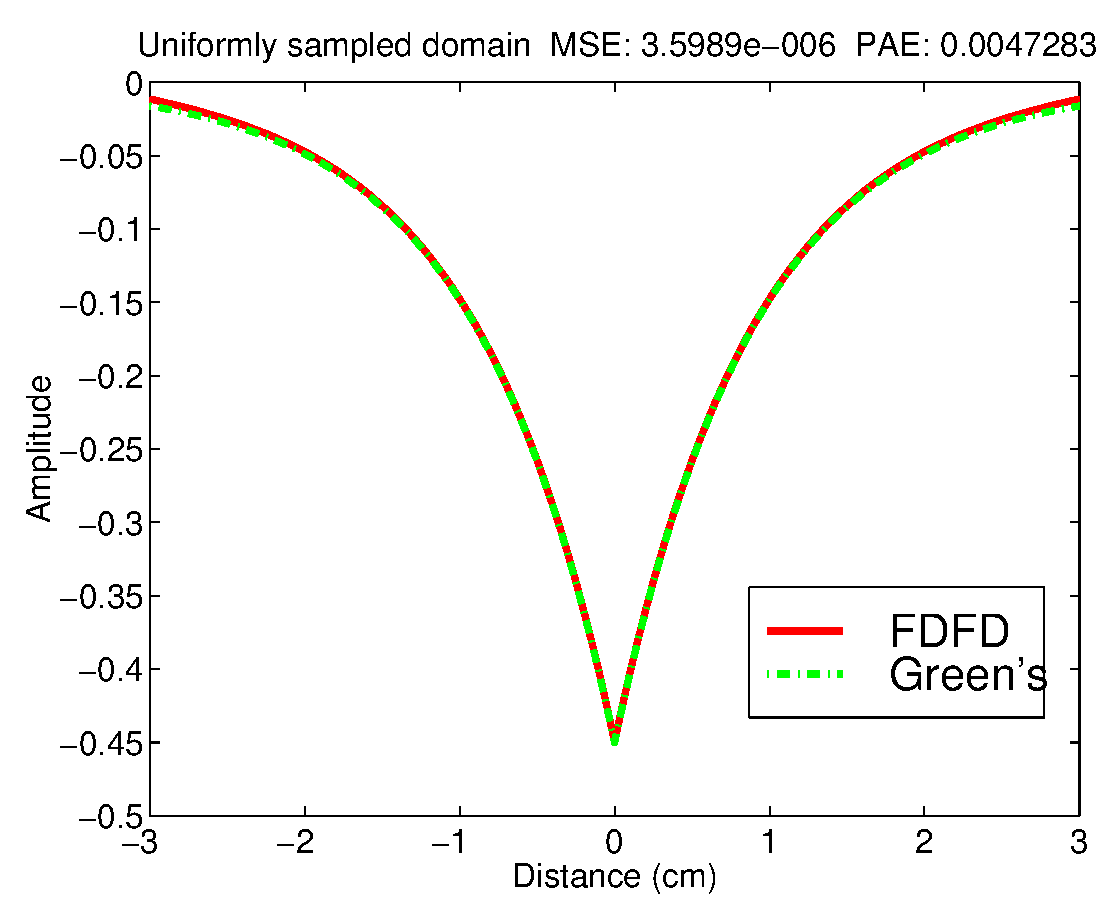
\includegraphics{unif1dex_0.eps}}
    \caption [uniform boundary 0 MHz] {Uniformly sampled FDFD and
    Green's functions solution to a single point source at the center
    of the region of interest.  The modulation frequency for the
    source was 0 MHz.}
\end {center}
\end {minipage}\hfill
\begin {minipage}[t]{3.0in}
    \begin {center}
    \scalebox{0.4}{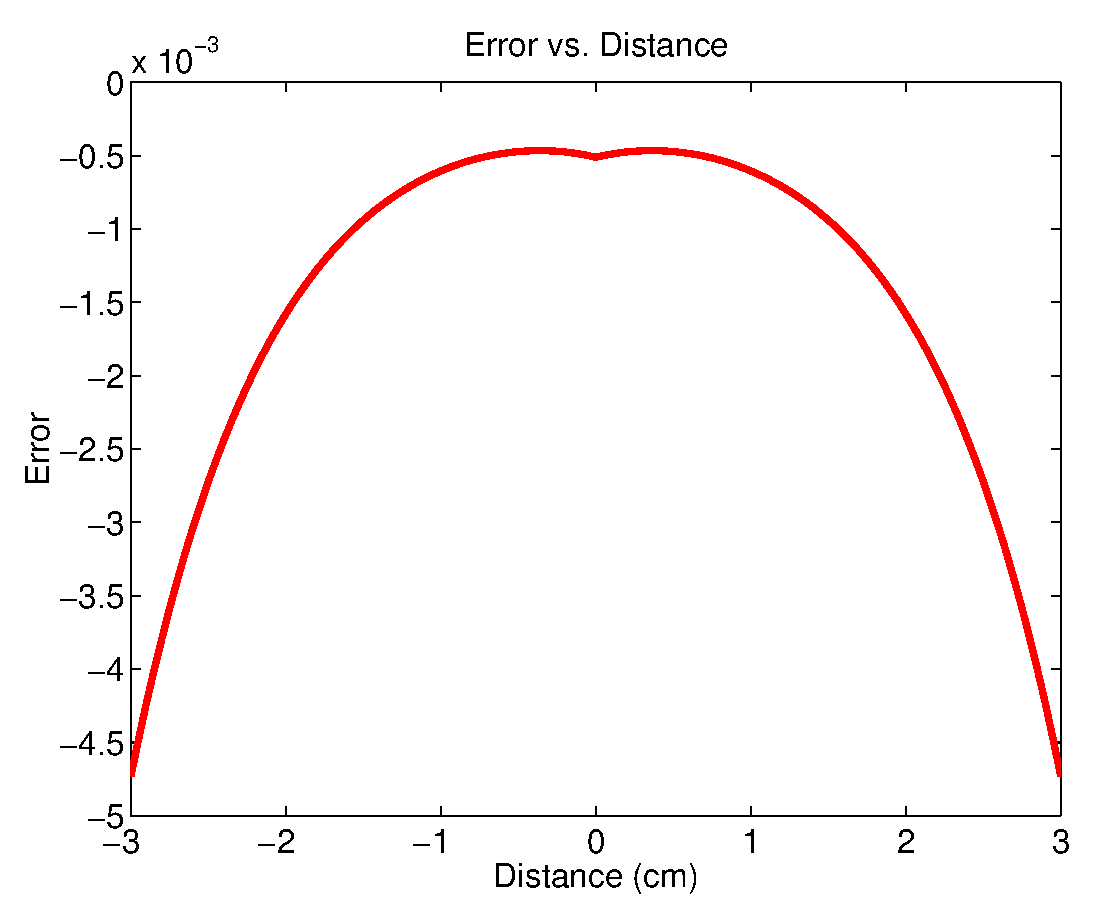
\includegraphics{unif1derr_0.eps}}
    \caption [uniform boundary error 0 MHz] {Error as a function of
    space for the uniformly sampled FDFD solution at 0 MHz.}
    \end {center}
\end {minipage}

\begin {minipage}[t]{3.0in}
    \begin {center}
    \scalebox{0.4}{\includegraphics{poly1dex_0.eps}} \caption
    [polynomial boundary 0 MHz] {Polynomially sampled boundary FDFD
    and Green's functions solution to a single point source at the
    center of the region of interest.  The modulation frequency for
    the source was 0 MHz.  The order of the polynomial was 4.3.}
\end {center}
\end {minipage}\hfill
\begin {minipage}[t]{3.0in}
    \begin {center}
    \scalebox{0.4}{\includegraphics{poly1derr_0.eps}} \caption
    [polynomial boundary error 200 MHz] {Error as a function of space
    for the polynomially sampled FDFD solution at 200 MHz.  Note that
    the range for this plot is an order of magnitude less than the
    corresponding uniformly sampled case above.}
    \end {center}
\end {minipage}
\end {figure}

Figures 5 through 8 show the same performance curves as Figures 1
through 4 but with a source modulation frequency of 200 MHz.  Again,
it is evident that the Polynomially sampled boundary significantly
outperforms the uniformly sampled boundary.  The mean squared error
for uniformly sampled boundary was 3.94E-7 while polynomially sampled
boundary had a mean squared error of 4.88E-9.   The peak absolute
error was 1.69E-3 and 2.27E-4 for the uniform and polynomial
boundaries respectively.  Thus, in both cases I observe almost an
order of magnitude improvement.  Even though the MSE improved almost 2
orders of magnitude a more appropriate measure for improvement would
be root-mean-squared-error which would show about an order of
magnitude improvement.

The 200 MHz case shows less improvement due to the polynomial boundary
compared to the 0 MHz case.  This can be explained by looking at the
imaginary part of the wavenumber for the two cases.  For 0 MHz it was
1.113 and for 200 MHz it was 1.2961.  This results in higher damping
for the 200 MHz case and therefore the computational boundary has less
of an affect on the error.

\begin {figure}
\begin {minipage}[t]{3.0in}
    \begin {center}
    \scalebox{0.4}{\includegraphics{unif1dex_200.eps}}
    \caption [uniform boundary 200 MHz] {Uniformly sampled FDFD and
    Green's functions solution to a single point source at the center
    of the region of interest.  The modulation frequency for the
    source was 0 MHz.}
\end {center}
\end {minipage}\hfill
\begin {minipage}[t]{3.0in}
    \begin {center}
    \scalebox{0.4}{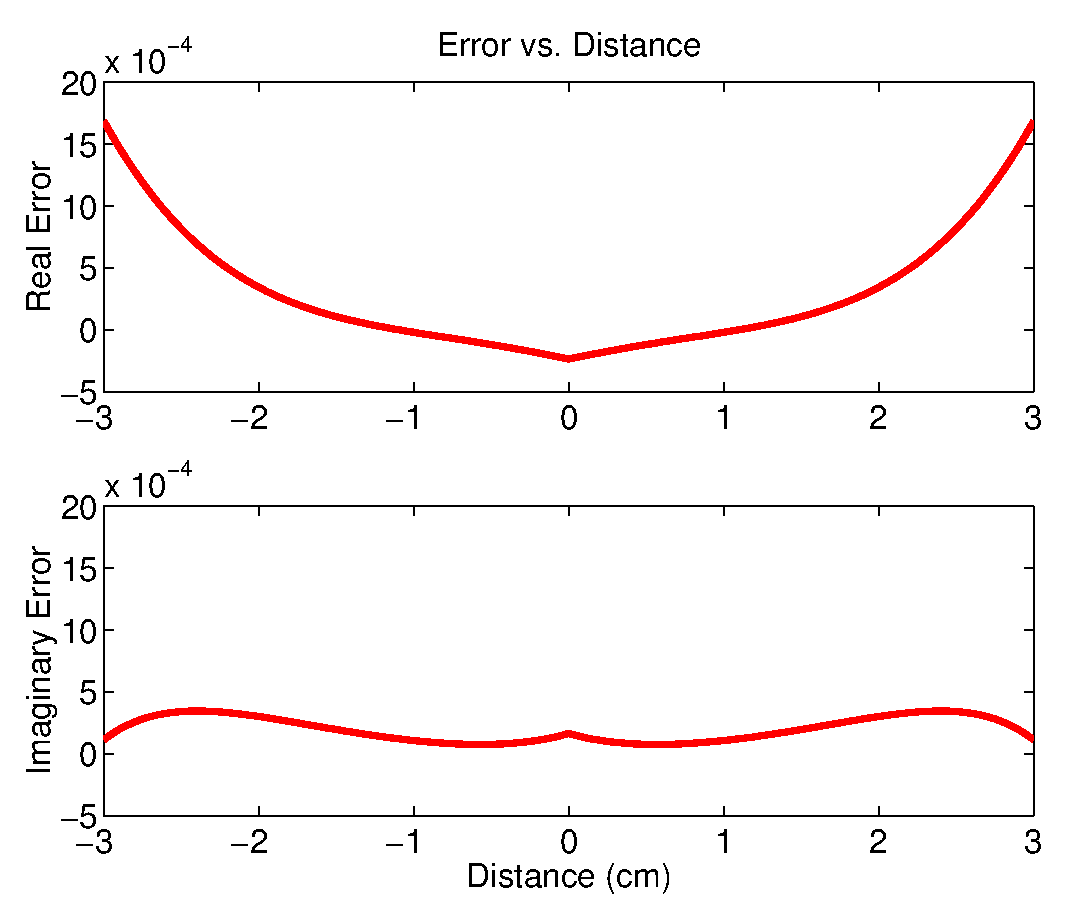
\includegraphics{unif1derr_200.eps}}
    \caption [uniform boundary error 200 MHz] {Error as a function of
    space for the uniformly sampled FDFD solution at 200 MHz.}
    \end {center}
\end {minipage}

\begin {minipage}[t]{3.0in}
    \begin {center}
    \scalebox{0.4}{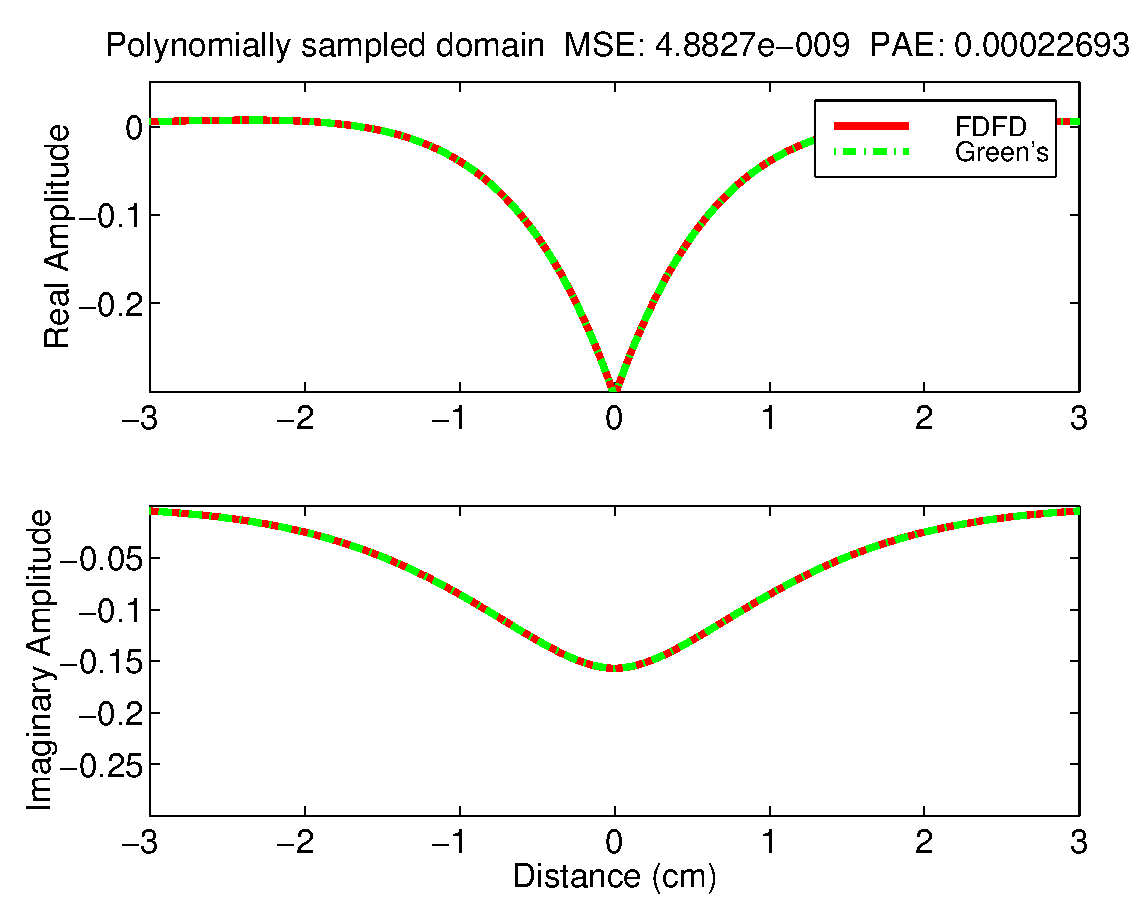
\includegraphics{poly1dex_200.eps}} \caption
    [polynomial boundary 200 MHz] {Polynomially sampled boundary FDFD
    and Green's functions solution to a single point source at the
    center of the region of interest.  The modulation frequency for
    the source was 200 MHz.  The order of the polynomial was 3.3.}
\end {center}
\end {minipage}\hfill
\begin {minipage}[t]{3.0in}
    \begin {center}
    \scalebox{0.4}{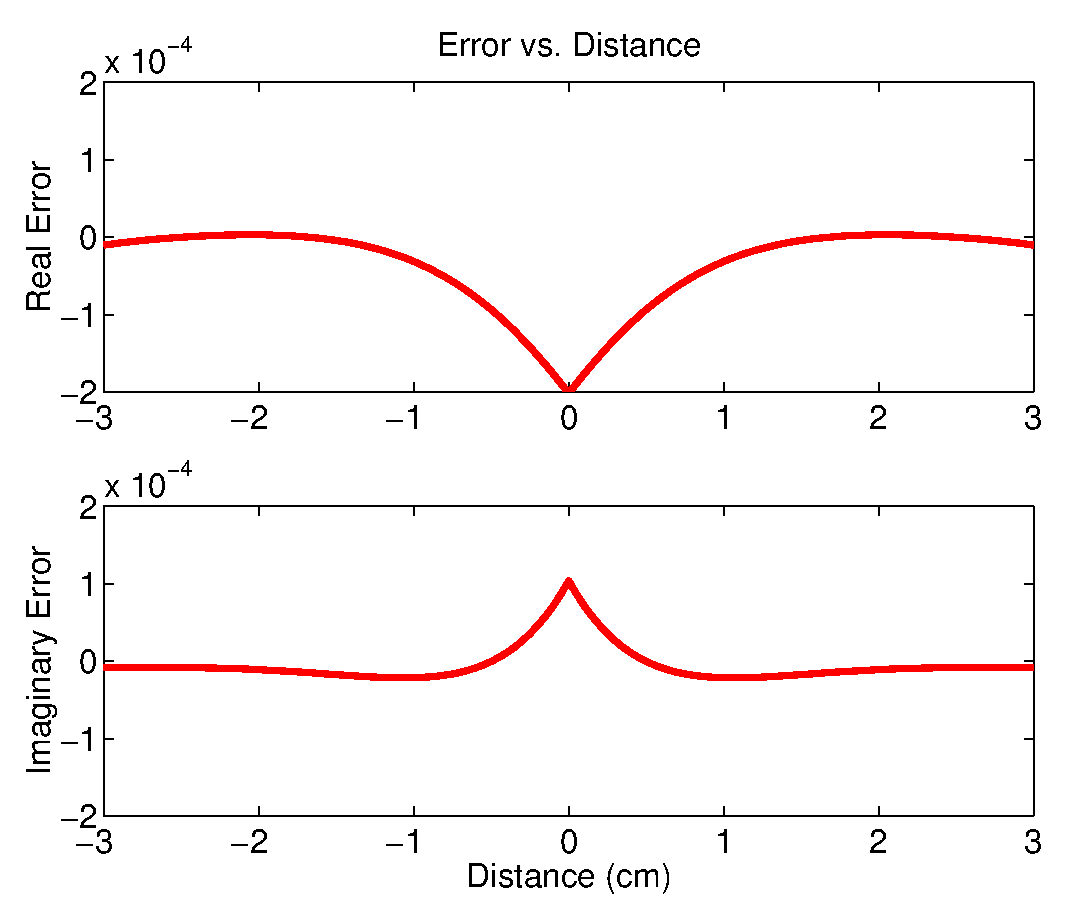
\includegraphics{poly1derr_200.eps}} \caption
    [polynomial boundary error 200 MHz] {Error as a function of space
    for the polynomially sampled FDFD solution at 200 MHz.  Note that
    the range for this plot is an order of magnitude less than the
    corresponding uniformly sampled case above.}
    \end {center}
\end {minipage}
\end {figure}

The next analysis I performed was to try to identify the optimal, in
the sense of minimizing the mean squared error in the region of interest,
polynomial order to use for the polynomial boundary.  This was
accomplished by plotting the mean squared error as a function of the
order parameter for both the 0 and 200 MHz cases.  The mean squared
error and peak absolute error versus order for the 0 MHz source
modulation case is shown in Figure 9.  It is evident from this figure
that a polynomial order of about 3 or 4 provides optimal performance
for this particular scenario.  Additionally, it is reassuring to note
minimum is fairly insensitive to the order parameter.  The order that
produced the minimum for this instance was 4.3.  Figure 10 shows the
same performance curves for the 200 MHz case.  Again, the optimum
region of was around an order of 3 to 4 and the was small sensitivity
to the order in this region.  The optimum value for the 200 MHz case
was 3.3.  Also, of note is the performance at an polynomial order of
1, this corresponds to the uniformly sampled case.  These graphs
clearly show the improvement in error performance over uniformly
sampled boundary region.

\begin {figure}
\begin {minipage}[t]{3.0in}
    \begin {center}
    \scalebox{0.4}{\includegraphics{ordereval_0.eps}} \caption
    [Order eval 0 MHz] {Error versus order of the polynomial
    approximation at 0 MHz.  The top graph shows the mean squared error and the
    bottom graph shows the peak absolute error as a function of
    polynomial order of the boundary elements.}
\end {center}
\end {minipage}\hfill
\begin {minipage}[t]{3.0in}
    \begin {center}
    \scalebox{0.4}{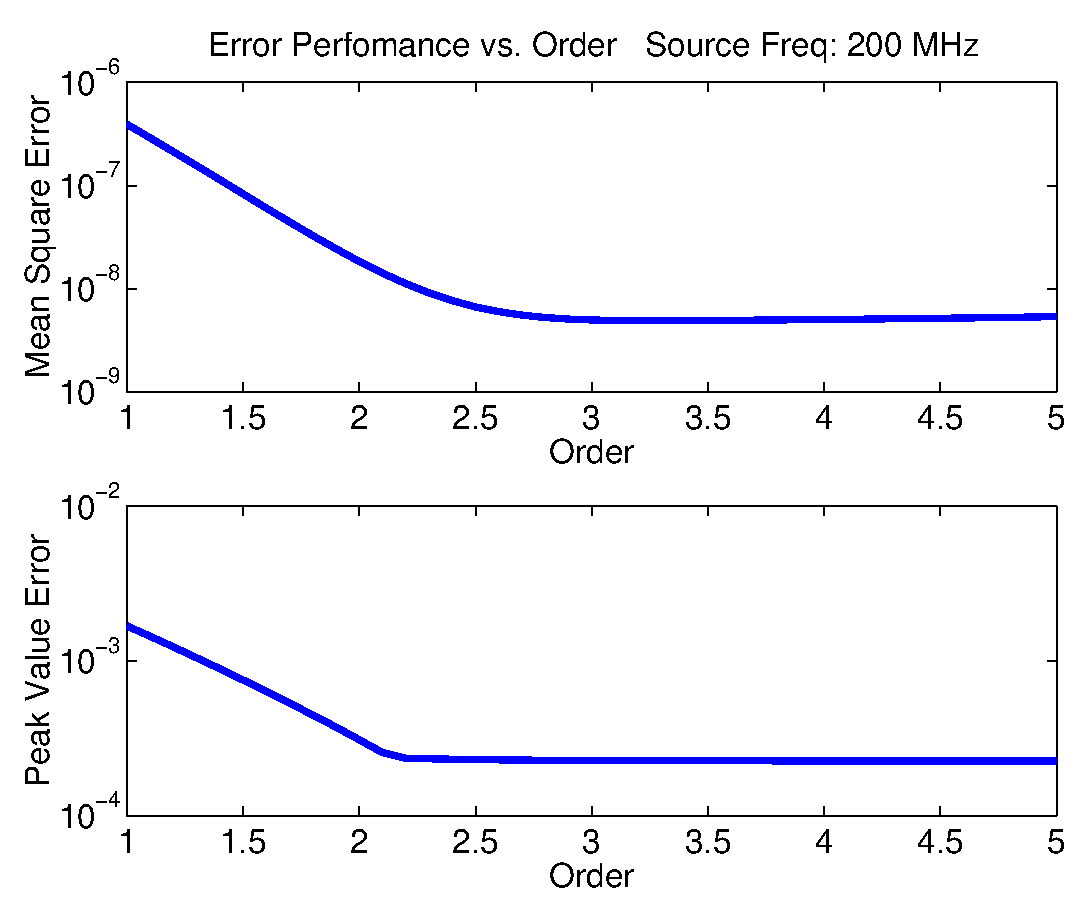
\includegraphics{ordereval_200.eps}} \caption
    [Order eval 200 MHz] {Error versus order of the polynomial
    approximation at 200 MHz.  This graph shows the same error
    measures as Figure 9.}
    \end {center}
\end {minipage}
\end {figure}

In effort to quantify the effect on the amount of computational work
saved I investigated how many samples of uniformly spaced boundary
were necessary to achieve the error performance of the polynomial
boundaries described above.  Recall that these scenarios had 121
samples in ROI and 10 samples on either side to implement the
boundary.  To achieve a mean squared error of 3.60E-3 for the 0 MHz
case a uniformly sampled boundary must have 56 samples for each
boundary.  This increases the total number of samples for the domain
from 141 to 233.  At 200 MHz the required number of of boundary
samples on each side for a uniformly sampled boundary to achieve the
performance of the 10 sample polynomial boundary was 48.  This
increases the total number of necessary samples in the domain from 141
to 217.  Thus, it is clearly evident that the polynomial boundary
technique provides a significant decrease in the amount of
computational work necessary.  This would become especially evident
when extending this method to three dimensions due to the cubic
increase in the size of the problem.

\section {Conclusions and future work}
\vspace {-4ex}
In this project I have presented a new technique for computing the
solution to a lossy Helmholtz equation in an unbounded domain.  With
minimal addition work up front computation of this problem can be
considerably reduced or equivalently accuracy can be enhanced.

Future work on this topic will include exploring in more detail how
the wavenumber affects the optimum selection of the order of the
polynomial.  Also, I will explore how the computational savings are
affected by fewer samples in the region of interest.  Since my
particular application is three-dimensional, I don't expect to be able
to compute a system with 120 samples per dimension.  Finally,
different functions in place of the polynomial, such as the
exponential, will be explored to evaluate their performance in this
scenario.
\bibliographystyle{unsrt}
\bibliography{EMAGProject}
\end {document}
